%% Revised IEEE conference paper. Development numbers come from the saved evidence package
%% (EV-xxx); prospective numbers come from EXP-063 run 2 (docs/EXPERIMENT_LOG.md,
%% seirgnn2/results/prospective_final.json and prospective_stats.json, data commit fc17870,
%% settings commit b248755). No unrun experiment or unsupported sensitivity analysis is reported.
\documentclass[conference]{IEEEtran}
\usepackage{cite}
\usepackage{amsmath,amssymb}
\usepackage{graphicx}
\graphicspath{{ieee/}{}}
\usepackage{booktabs}
\usepackage{url}

\hyphenation{epi-demi-o-log-i-cal}

\begin{document}

\title{SEIR-Informed Graph Forecasting for Dengue: \\ A Development Gain That Did Not Survive Prospective Evaluation}

\author{\IEEEauthorblockN{Tharusha Perera, Praveen De Silva, Janith Mahanama,
Bimsara Udurawana, \\
Maleesha Kumarasinghe, Praveen Nawarathna}
\IEEEauthorblockA{Department of Computer Science and Engineering, University of Moratuwa\\
Moratuwa, Sri Lanka\\
\{tharushap.23, praveend.23, janithm.23, bimsarau.23,\\
kumarasinghemp.23, praveenn.23\}@cse.mrt.ac.lk}}

\maketitle

\begin{abstract}
We study a hybrid forecaster that couples an adaptive graph encoder to a susceptible--exposed--infectious--recovered (SEIR) decoder, with a population-and-susceptibility anchored transmission rate and a learned gate to persistence, for three-week-ahead dengue forecasts in 25 Sri Lankan districts.
On a reconstructed series of 559 weekly reports (2013--2024), the model had the lowest point-estimate RMSE among 30 learned configurations over nine development origins, 27.45 versus 28.54 for persistence, without statistical support. % EV-200, EV-215, EV-219
We then froze the models, tuning budget, baselines and analysis in a committed plan before parsing 127 later reports (March 2024 to August 2026), corrected the district graph, removed target overlap between partitions, and added a matched gated non-SEIR control and seasonal-naive and autoregressive baselines.
After three documented corrections to how the new weeks were reconstructed, one of which invalidated a first run, the amended prospective evaluation on 85 forecast starts found the lowest RMSE for persistence, 34.75. % EXP-063 run 2
The SEIR model (35.40) did not differ from its matched non-SEIR control (35.43; difference $-0.03$, 95\% interval $-0.41$ to $0.12$, Holm-adjusted $p=0.67$) and did not beat persistence ($+0.65$, $-0.99$ to $1.69$, $p=0.62$). % EXP-063 run 2
Mechanistic SEIR constraints were therefore feasible but did not improve prospective RMSE; source checking and prospective evaluation materially changed the interpretation of the development results.
\end{abstract}

\begin{IEEEkeywords}
dengue forecasting, epidemic modeling, graph neural networks, persistence baseline, prospective evaluation, SEIR model
\end{IEEEkeywords}

\section{Introduction}
Dengue causes recurring epidemics in Sri Lanka~\cite{tissera2020severe}.
Short-horizon district forecasts can support planning for clinical capacity and vector-control activity.
Spatio-temporal graph models are attractive because districts are not independent: neighbouring areas can share mobility, environmental conditions, and reporting patterns~\cite{weng2024graph}.
Their learned dynamics, however, need not respect the latent exposed and infectious stages that constrain how incidence can evolve.
Compartmental models encode this structure: an SEIR model tracks movement through susceptible, exposed, infectious, and recovered states, and Liu et al.~\cite{liu2025seirlstm} showed that a neural model can learn the force of infection for Sri Lankan dengue.

We ask whether an SEIR-informed decoder integrated with a graph forecaster improves on a matched graph-only model and on persistence, the forecast that repeats the latest week.
Persistence is essential because weekly dengue counts change gradually over short horizons, and the earlier Sri Lankan graph benchmark does not report it~\cite{weng2024graph}.

This study makes four contributions.
First, we construct a hybrid graph--SEIR forecaster whose transmission rate is anchored to district population and susceptible fraction and whose output can fall back to persistence through a learned gate.
Second, we rebuild and source-check the district surveillance series and show that one spreadsheet error materially changes the apparent difficulty of the legacy benchmark.
Third, we evaluate 30 learned configurations over nine rolling development origins, where the hybrid model shows a small, statistically unsupported lead.
Fourth, we test that lead in a prospective evaluation on 127 later weekly reports whose design was committed before the new reports were parsed; the lead does not survive.

\section{Related Work}
Weng et al.~\cite{weng2024graph} adapted several graph encoders to Sri Lankan dengue forecasting, including STGAT, A3T-GCN, ASTGCN, DCRNN, and AAGCN~\cite{huang2019stgat,bai2021a3tgcn,guo2019astgcn,li2018dcrnn,shi2019aagcn}.
DengueGNN also studies graph-based dengue prediction~\cite{gulmohamed2026denguegnn}, while Graph WaveNet introduced the learned-adjacency construction used in our adaptive encoder~\cite{wu2019graphwavenet}.
Liu et al.~\cite{liu2025seirlstm} combine neural prediction with a human SEIR model for dengue in Sri Lanka.
EINNs and CausalGNN incorporate epidemiological assumptions into neural forecasters, and MepoGNN couples graph learning with metapopulation epidemic dynamics~\cite{rodriguez2023einns,wang2022causalgnn,cao2023mepognn}.
We test their combination against persistence and a matched non-SEIR control on later data.

\section{Data}\label{sec:data}
\subsection{Development series}
The reconstructed development series contains 559 weekly reports for 25 districts from June 15, 2013, to February 24, 2024; seven reports are missing and are left missing. % EV-216
Any forecast window whose inputs or targets touch a missing report is excluded.
Each forecasting sample maps the previous three weeks of district counts to the next three weeks. % EV-007
The earlier benchmark array, referred to here as the legacy array, contains 459 rows without a verified calendar. % EV-002

\begin{figure}[t]
\centering
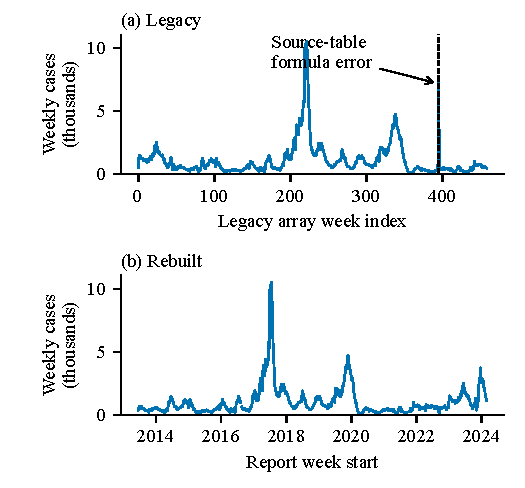
\includegraphics[width=\columnwidth]{figures/fig_data.pdf}
\caption{National weekly cases summed over 25 districts. (a) Legacy benchmark array, with the source-table formula error marked. (b) Reconstructed development series; gaps denote missing reports. The prospective period (Section~\ref{sec:prospective}) follows (b).}
\label{fig:data}
\end{figure}

During reconstruction, each district row was checked against the printed national total.
Legacy row 395 corresponds to the report for December 26, 2020, to January 1, 2021~\cite{epid2021wer0248}. % EV-222
In its weekly row, 15 of 24 inner cells equal the sum of the two preceding cells; the district entries sum to 7165 while the printed weekly national total is 35. % EV-222
The same report's year-to-date row is consistent with its printed total of 351 when Kalmunai is included, so we treat the legacy spike as a spreadsheet formula error rather than an outbreak and use the year-to-date row for that report. % EV-222

\subsection{Prospective series}
The 127 Weekly Epidemiological Reports that follow the development series (Vol.~51 No.~11 to Vol.~53 No.~33, printed weeks starting March 2, 2024, to August 3, 2026) were downloaded and checksummed, and their correction rules were committed before any count was parsed. % EXP-063
A week's count is the report's weekly row if its districts and Kalmunai sum to the printed national total and it does not show the formula pattern above; otherwise it is the difference of year-to-date rows, if that passes the same checks; otherwise the week is missing.
Nothing is interpolated.
Three corrections to this reconstruction are described with the evaluation in Section~\ref{sec:deviations}.
The final prospective series has 109 weeks taken as printed, 8 recovered from year-to-date rows, and 10 missing. % EXP-063, data commit fc17870

\subsection{Spatial graph}
Districts are graph nodes and shared borders define the static adjacency.
Checking the border list against GADM polygons gives 57 shared borders, 114 directed entries, and 139 entries after self-loops. % EV-221
The saved development experiments used the benchmark graph, which contains two additional one-directional entries, Kandy--Ampara and Kegalle--Kalutara, that are not shared borders, for 141 entries. % EV-221
We keep those historical scores for traceability; the prospective evaluation and its tuning runs use the corrected 139-entry graph.

\section{SEIR-Informed Graph Network}\label{sec:methods}
Fig.~\ref{fig:arch} summarizes the model.
The graph encoder captures inter-district dependence, while the decoder constrains within-district trajectories through daily compartment flows.
For each district and forecast horizon, the encoder produces a read-out $r$ that is mapped either directly to a forecast or to parameters of the SEIR head.

\begin{figure*}[t]
\centering
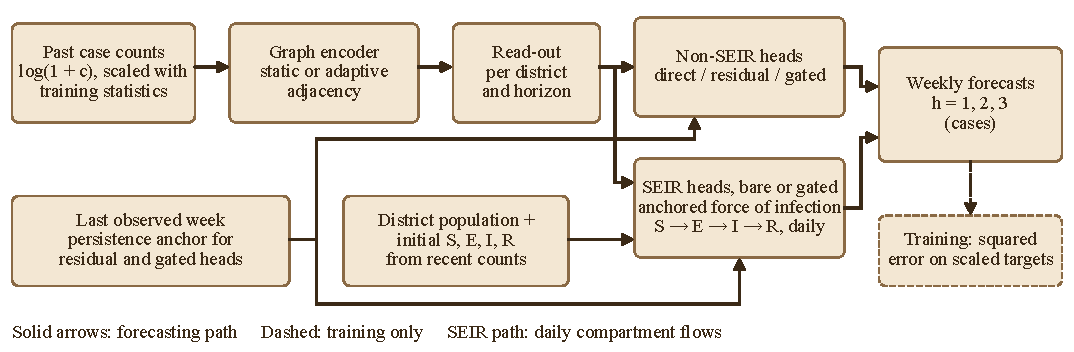
\includegraphics[width=\textwidth]{figures/fig_arch.pdf}
\caption{SEIR-informed graph network. The graph encoder and read-out feed either a non-SEIR head or an SEIR head that converts a learned force of infection into weekly incidence through daily compartment flows. Residual and gated heads use the last observed week as a persistence anchor.}
\label{fig:arch}
\end{figure*}

\subsection{Encoder and prediction heads}
Counts $c_{i,t}$ for district $i$ and week $t$ are transformed using training-period statistics,
\begin{equation}
z_{i,t}=\{\log(1+c_{i,t})-\mu\}/\sigma.
\label{eq:z}
\end{equation}
The persistence anchor $p$ repeats the standardized latest count at all three horizons.
The GCN encoder projects the input to a hidden width (64 unless stated) and applies two residual graph layers, $H'=H+\mathrm{Dropout}(\mathrm{ReLU}(AHW+b))$, where $A$ is the row-normalized adjacency with self-loops. % EV-177
The adaptive encoder learns $A_{\rm ad}=\mathrm{softmax}(\mathrm{ReLU}(E_1E_2^\top))$ from standard-normal $25\times10$ node embeddings shared by both layers and excluded from weight decay. % EV-177

A direct head outputs $r$; a residual head outputs $p+r$; and a gated head learns how far to move from persistence, $p+g(r-p)$, with $g=\mathrm{sigmoid}(a)$ and $a$ initialized at $-2$. % EV-178
The bare SEIR head outputs the standardized simulator count $z(\hat c)$, while the gated SEIR head outputs $p+g\{z(\hat c)-p\}$ with the same gate and initialization, so the gated non-SEIR head is its matched control.
All learned models minimize squared error on the standardized log scale; count-scale RMSE is an evaluation metric rather than the quantity directly optimized.

\subsection{SEIR decoder}
For each horizon, the decoder advances susceptible, exposed, infectious, and recovered fractions one day at a time,
\begin{equation}
\begin{aligned}
f_S&=S(1-e^{-\lambda\Delta t}),\quad f_E=E(1-e^{-\omega\Delta t}),\\
f_I&=I(1-e^{-\gamma\Delta t}),\quad
\hat c_{i,h}=\rho_{\rm eff}N_i\sum_{d=1}^{7} f_E^{(d)}.
\end{aligned}
\label{eq:seir}
\end{equation}
Flows are computed from the current state and moved along $S\rightarrow E\rightarrow I\rightarrow R$; predicted weekly cases are the daily exposed-to-infectious flows summed over seven days and scaled by district population $N_i$ and an effective reporting fraction.
We use $\omega=0.7/7=0.1$ and $\gamma=1/7$ per day, corresponding to mean exposed and infectious periods of ten and seven days, following Liu et al.~\cite{liu2025seirlstm}. % EV-011
The base reporting fraction is $\rho=1/11$, with a learned global multiplier $\rho_{\rm eff}=\rho\exp(q)$. % EV-011, EV-217
Initial infectious and exposed fractions are derived from $c_{t-1}/(\rho N_i)$ and $c_{t-2}/(\rho N_i)$ and clipped to $[10^{-6},0.5]$. % EV-170
The susceptible fraction is $\mathrm{clip}(0.318-C_{<t}/(\rho N_i),0.01,1)$, where $C_{<t}$ is the cumulative earlier report count, and 0.318 is one minus the 68.2\% seroprevalence measured in suburban Colombo~\cite{jeewandara2015sero}, applied to every district. % EV-170, EV-223
A multiplier $2\,\mathrm{sigmoid}(v)$ rescales the exposed fraction, either globally or per district from the encoder. % EV-217

The force of infection is either free or anchored.
The free rate exponentiates the read-out plus a learned bias.
The anchored rate supplies an epidemiological scale before the learned adjustment,
\begin{equation}
\lambda^*_{i,h}=\frac{\max(c_{i,t-1},0.5)}{7\rho_{\rm eff}N_iS_i}
\exp\{\mathrm{clip}(r_{i,h},-10,10)\},
\label{eq:anchor}
\end{equation}
the daily rate that would reproduce last week's reported count, times a learned multiplicative departure.
Both rates are multiplied by a learned spatial import term $\exp\{0.1\beta(u_i-\bar u)\}$, where $u_i=\log\max((AI)_i,10^{-9})$. % EV-217
A mass-action ablation instead uses a learned daily transmission coefficient times the infectious fraction, recomputed each day.
We refer to the adaptive encoder with the gated anchored SEIR head and encoder-derived $E_0$ as the \emph{Adaptive SEIR-GNN}.

\section{Development Evaluation}\label{sec:setup}
\begin{figure}[t]
\centering
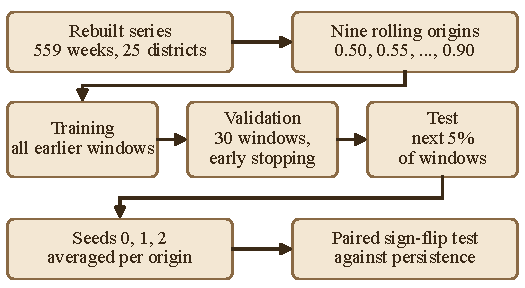
\includegraphics[width=\columnwidth]{figures/evaluation_protocol.pdf}
\caption{Development evaluation. At each of nine origins, models are trained on earlier windows, early-stopped on 30 validation windows, and scored on the next 5\% of forecast starts. Seed-averaged origin scores are paired with persistence.}
\label{fig:protocol}
\end{figure}

We use rolling-origin evaluation (Fig.~\ref{fig:protocol}) with nine cut-offs from 0.50 to 0.90 of the valid forecast-start list in steps of 0.05; each held-out block contains the next 5\% of starts, and the 30 starts before each cut-off form the validation set. % EV-186, EV-182
This grid was selected after earlier development runs, so it is not a preregistered test. % EV-227
Each learned configuration is trained with seeds 0, 1, and 2; persistence is deterministic. % EV-101
All learned models use Adam with learning rate 0.003 and weight decay 0.0001, batch size 32, cosine decay, gradient clipping at 5, at most 300 epochs, and early stopping on count-scale validation RMSE with patience 40. % EV-175, EV-224
Because every start predicts three weeks, adjacent partitions share two target weeks in this protocol, so early stopping sees outcomes that also occur in the first held-out windows. % EV-218
The 30 learned configurations are GCN, LSTM, STGAT, A3T-GCN, ASTGCN, and AAGCN with direct, residual, free-rate gated-SEIR, and bare-SEIR heads, plus six adaptive/anchored variants. % EV-179
Seeds are averaged within origin; each configuration is paired with persistence over the nine origins with a descriptive 95\% $t$ interval and an exact sign-flip test, Holm-adjusted across the 30 comparisons. % EV-200, EV-219
With nine origins, the smallest attainable Holm-adjusted $p$ is 0.117. % EV-226

\begin{table*}[t]
\centering
\caption{Development results on the rebuilt series (nine rolling origins, three seeds; benchmark graph, unpurged splits). These are not the prospective results of Table~\ref{tab:prospective}. RMSE and MAE are in cases per district-week, averaged over origins and seeds; horizon columns report RMSE. $\Delta$ is the seed-averaged paired RMSE difference from persistence with a 95\% t interval over origins (negative is better). Bold marks the lowest test RMSE (the proposed Adaptive SEIR-GNN); an interval that includes zero shows no clear difference from persistence.}
\label{tab:main}
\small\setlength{\tabcolsep}{3pt}
\begin{tabular}{@{}p{2.85in}rrrrrr@{}}
\toprule
Model & $h=1$ & $h=2$ & $h=3$ & RMSE & MAE & $\Delta$ [95\% CI] \\
\midrule
Persistence (last week) & 23.47 & 27.94 & 33.26 & 28.54 & 13.94 & -- \\ % EV-200

GCN, direct & 23.10 & 27.82 & 32.68 & 28.17 & 13.66 & -0.37 [-1.88, +1.14] \\ % EV-201

GCN, residual (baseline GNN) & 23.24 & 27.79 & 32.47 & 28.12 & 13.62 & -0.42 [-1.54, +0.70] \\ % EV-202

LSTM, direct & 23.65 & 28.22 & 33.38 & 28.73 & 14.00 & +0.19 [-1.99, +2.37] \\ % EV-203

ASTGCN, direct & 23.92 & 28.54 & 33.45 & 28.94 & 14.27 & +0.40 [-2.02, +2.81] \\ % EV-204

AAGCN, direct & 24.11 & 29.10 & 33.66 & 29.26 & 14.06 & +0.72 [-1.57, +3.00] \\ % EV-205

STGAT, direct & 42.60 & 44.55 & 46.75 & 44.71 & 22.17 & +16.17 [+4.24, +28.11] \\ % EV-206

ASTGCN, residual & 23.07 & 28.08 & 33.66 & 28.65 & 13.98 & +0.11 [-1.68, +1.90] \\ % EV-207

Adaptive GCN, residual & 23.07 & 27.78 & 32.15 & 27.94 & 13.61 & -0.60 [-1.81, +0.61] \\ % EV-208

GCN, SEIR, free rate & 27.58 & 40.81 & 50.14 & 40.77 & 17.97 & +12.23 [+2.67, +21.80] \\ % EV-209

GCN, gated SEIR, free rate & 22.86 & 28.04 & 33.29 & 28.43 & 13.51 & -0.11 [-3.23, +3.00] \\ % EV-210

Adaptive GCN, SEIR, anchored & 23.99 & 28.81 & 35.29 & 29.80 & 13.84 & +1.26 [-1.47, +3.98] \\ % EV-211

Adaptive GCN, gated SEIR, mass-action & 22.90 & 28.02 & 33.19 & 28.39 & 13.52 & -0.16 [-3.16, +2.85] \\ % EV-212

GCN, gated SEIR, anchored & 22.49 & 27.38 & 32.04 & 27.62 & 13.39 & -0.92 [-2.60, +0.76] \\ % EV-213

Adaptive GCN, gated SEIR, anchored & 22.51 & 27.09 & 31.85 & 27.45 & 13.31 & -1.09 [-2.81, +0.63] \\ % EV-214

\textbf{Adaptive GCN, gated SEIR, anchored, learned $E_0$} & \textbf{22.45} & \textbf{27.07} & \textbf{31.88} & \textbf{27.45} & \textbf{13.29} & \textbf{-1.10 [-2.84, +0.65]} \\ % EV-215

\bottomrule
\end{tabular}
\end{table*}


\subsection{Development results}
Persistence yields RMSE 28.54 and MAE 13.94, and the GCN residual baseline 28.12 and 13.62 (Table~\ref{tab:main}). % EV-200, EV-202
The Adaptive SEIR-GNN gives the lowest point-estimate RMSE, 27.45, a mean paired difference of $-1.10$ with 95\% interval $[-2.84, 0.65]$, raw $p=0.199$ and Holm-adjusted $p=1.000$; no configuration differs significantly from persistence. % EV-215, EV-219
It is below persistence at seven of nine origins, but variation between epidemic periods is far larger than the gap. % EV-114
Within the SEIR family, anchoring the rate lowers the GCN gated SEIR head from 28.43 to 27.62, and the bare anchored head (29.80) is worse than persistence while its gated version reaches 27.45 (Fig.~\ref{fig:results}b). % EV-210, EV-213, EV-211, EV-214
An adaptive residual model without a simulator reaches 27.94. % EV-208
These development comparisons lack a matched gated non-SEIR control, which the prospective evaluation adds.

\begin{figure*}[t]
\centering
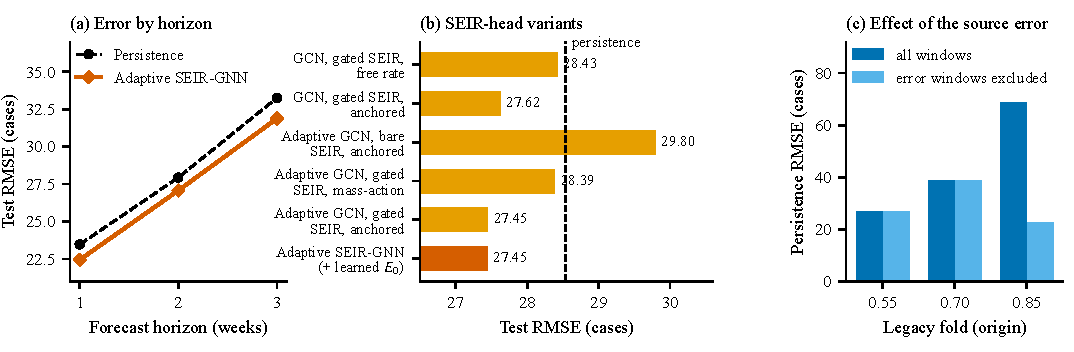
\includegraphics[width=\textwidth]{figures/fig_results.pdf}
\caption{(a) RMSE by forecast horizon. (b) SEIR-head ablations; the dashed line is persistence. (c) Persistence RMSE on the three legacy folds with all windows and after excluding the six windows that touch the erroneous source row. Panels (a) and (b) use the nine-origin development protocol.}
\label{fig:results}
\end{figure*}

On the legacy array, excluding the six windows that touch the erroneous report lowers mean persistence RMSE from 44.80 to 29.52 (Fig.~\ref{fig:results}c), far more than the 1.10-case gap between the best learned configuration and persistence. % EV-220, EV-215

\section{Prospective Evaluation}\label{sec:prospective}
\subsection{Frozen design}
Before any new report was parsed, we committed a plan fixing the arms, tuning budget, splits, metrics, tests and the claims each result would permit. % EXP-063, plan commit 92952ba
It was amended once, still before parsing, on external review: the autoregressive baseline was made recursive and the bootstrap sensitivity block lengths were set to 4 and 12. % EXP-063, plan amendment 1, 3317bda
The arms are the Adaptive SEIR-GNN; its matched control, the same adaptive encoder with the gated non-SEIR head; the adaptive residual model; persistence; a seasonal-naive forecast that repeats the count 52 weeks before each target (persistence where that week is missing); and a pooled recursive AR(3) ridge regression on $\log(1+c)$ with district intercepts.
All learned arms use the corrected graph.

To remove target overlap, the last $H-1=2$ forecast starts before each partition boundary are dropped, so no target week belongs to two partitions.
Each neural arm received the same validation-only tuning budget, learning rate $\{0.001, 0.003\}$ by hidden width $\{32, 64\}$, chosen by mean validation RMSE over the nine purged development origins and three seeds; all three chose 0.003 and 64. % EXP-063, b248755
The AR penalty was chosen from five values on the same splits.
The final split trains on 486 development starts, early-stops on the last 30, and tests on every start whose three targets lie in the prospective period; each arm is trained once per seed and applied to the whole period without refitting. % EXP-063 run 2

The inference unit is the forecast start: its 25 districts and three horizons stay together.
For each start, the squared error is averaged over districts, horizons and seeds; RMSE differences are resampled with a paired circular moving-block bootstrap~\cite{kunsch1989bootstrap,politis1992circular} with blocks of 8 starts and 10{,}000 replicates.
The two primary comparisons, the SEIR model against its matched control (P1) and against persistence (P2), are Holm-adjusted.
The plan permits a claim of improvement only for an adjusted $p<0.05$ in the model's favour.

\subsection{Reconstruction corrections and the invalid first run}\label{sec:deviations}
The first parse marked every report missing because PDF extraction adds an empty trailing column to otherwise valid tables; the parser was corrected to remove trailing blank cells only and to validate all 27 column labels before reading any count (amendment 1). % EXP-063, 9125c0f
A first prospective run on the resulting series gave every arm an RMSE near 284. % EXP-063 run 1, 708f290
This exposed two reconstruction defects, not model behaviour.
In these volumes report No.~$N$ carries printed week $N-1$, so the rule that the year-to-date row of report No.~1 is a weekly count instead entered a whole year's total, 50{,}052 cases, as one week; and two reports reprint the previous week's table.
Amendment 2 keys the year-to-date rule on the printed week, treats a repeated weekly row as failed, never uses a negative difference, and logs cross-week checks; amendment 2b marks a week missing when its year-to-date difference merely reproduces a repeated row. % EXP-063, bd26f2a, 05f95eb, 63d2432
No rule limits the size of a weekly count, and no model setting changed after tuning.
The first run is invalid and is reported only as this deviation; because it had already shown horizon-one errors close to persistence for all arms, the second run is an amended prospective evaluation following a data-quality correction, not a fully untouched test.

\begin{table*}[t]
\centering
\caption{Prospective results (run 2): 85 forecast starts with all targets between March 2024 and June 2026, settings frozen before the period was parsed. Learned arms are averaged over seeds 0, 1, 2; their seed RMSE ranges are 0.45 (SEIR), 0.36 (gated) and 0.82 (residual). $\Delta$ is the RMSE difference from persistence with a 95\% paired circular block-bootstrap interval over forecast starts (block 8; negative favours the model). MAE, SMAPE and MAPE are descriptive and were not tested. Bold marks the lowest value in each column.}
\label{tab:prospective}
\small\setlength{\tabcolsep}{3.5pt}
\begin{tabular}{@{}lrrrrrrrl@{}}
\toprule
Model & $h=1$ & $h=2$ & $h=3$ & RMSE & MAE & SMAPE & MAPE & $\Delta$ [95\% CI] \\
\midrule
Persistence (last week) & \textbf{15.40} & 35.66 & \textbf{45.98} & \textbf{34.75} & 11.78 & 50.25 & 53.30 & -- \\ % EXP-063 run 2
Seasonal naive (52 weeks earlier) & 50.72 & 62.46 & 72.24 & 62.43 & 27.53 & 74.63 & 113.35 & +27.68 [+14.08, +48.35] \\ % EXP-063 run 2
AR(3), recursive ridge & 17.33 & 35.87 & 48.75 & 36.35 & 11.35 & 46.75 & 44.46 & +1.60 [-1.21, +3.09] \\ % EXP-063 run 2
Adaptive GCN, residual & 16.37 & 36.02 & 47.61 & 35.74 & 11.61 & 46.61 & \textbf{43.01} & +0.99 [-0.44, +2.54] \\ % EXP-063 run 2
Adaptive GCN, gated non-SEIR (matched control) & 16.01 & 35.66 & 47.31 & 35.43 & 11.35 & \textbf{45.75} & 43.91 & +0.68 [-0.69, +1.85] \\ % EXP-063 run 2
Adaptive SEIR-GNN & 15.78 & \textbf{35.65} & 47.32 & 35.40 & \textbf{11.29} & 46.08 & 43.47 & +0.65 [-0.99, +1.69] \\ % EXP-063 run 2
\bottomrule
\end{tabular}
\end{table*}


\subsection{Prospective results}
Table~\ref{tab:prospective} reports the second run on 85 forecast starts. % EXP-063 run 2
Persistence has the lowest RMSE, 34.75.
The Adaptive SEIR-GNN (35.40) and its matched gated non-SEIR control (35.43) are essentially identical: the P1 difference is $-0.03$ with 95\% interval $[-0.41, 0.12]$ and Holm-adjusted $p=0.67$. % EXP-063 run 2
Against persistence the SEIR model is $+0.65$ worse, $[-0.99, 1.69]$, adjusted $p=0.62$ (P2). % EXP-063 run 2
Block lengths 4 and 12 give the same conclusions (P1 $p=0.68$ and $0.66$; P2 $p=0.24$ and $0.32$). % EXP-063 run 2
Neither claim permitted by the plan is supported.

The learned arms have lower MAE, SMAPE and MAPE than persistence, for example MAE 11.29 versus 11.78 for the SEIR model; these metrics were not primary and were not tested, so we report them descriptively. % EXP-063 run 2
In secondary, unadjusted comparisons, both gated arms beat the adaptive residual model (SEIR $-0.34$, $[-1.00, -0.08]$), every arm beats seasonal naive, and AR(3) does not differ clearly from persistence or the learned arms. % EXP-063 run 2

High-incidence weeks dominate the score.
Only 3 of the 85 starts fall in 2026, when weekly national counts reach 7{,}279 against a 2025 median of 926, yet they account for about three quarters of the squared error for persistence and for the SEIR model alike. % EXP-063 run 2, losses by start
We do not attribute the result to that outbreak; it means that RMSE over this period mostly measures a few large weeks, on which no arm separates from persistence.

The development and prospective evidence also disagree in an informative way.
In the purged development runs used for tuning, the SEIR model led its matched control on the development test blocks (27.34 versus 27.90) but not on validation (24.92 versus 24.90); the later period agrees with validation. % EXP-063 step 3, prospective_dev.json

\section{Discussion and Limitations}\label{sec:discussion}
The development lead of the hybrid model did not generalize.
On later data, the SEIR equations added nothing measurable over an identical gated model without them, and no learned model improved RMSE over persistence.
The development results remain useful as a map of what fails: a bare simulator is worse than persistence, and the gate to persistence is what keeps the SEIR head competitive.
That the gated model with and without SEIR coincide prospectively suggests the gate, not the compartment equations, carried most of the SEIR head's development performance.
Weekly dengue counts are strongly persistent over three weeks, which leaves little room for any model unless it anticipates changes that recent counts do not show.

Source checking changed the conclusions twice.
One formula error moves the legacy persistence benchmark by more than the entire gap among the strongest models, and the prospective reconstruction needed three corrections, one of which turned a meaningless run into a valid one.
Benchmarks assembled from public surveillance reports need cross-week checks, not only checks within each table.

Several limitations remain.
The prospective evaluation was amended after a first run had been scored, so it is not fully blind, although every correction concerns data reconstruction and the models were frozen beforehand.
It covers one period with 85 forecast starts, and its RMSE is dominated by three high-incidence starts; ten prospective reports are missing.
The tuning budget was small, the same for every neural arm, and the earlier development grid shared target weeks across partitions and used a graph with two non-border entries.
The SEIR decoder uses fixed disease durations, a learned scaling of a base reporting fraction, a Colombo-derived susceptible fraction for every district, and no mosquito, serotype or waning-immunity compartments; we did not test sensitivity to these choices and make no robustness claim.

\section{Conclusion}
We built an SEIR-informed graph forecaster for weekly district dengue in Sri Lanka and tested it first on development data and then prospectively on 127 later weekly reports under a design committed in advance.
In development it recorded the lowest RMSE, 27.45 versus 28.54 for persistence, without statistical support. % EV-200, EV-215, EV-219
Prospectively, persistence had the lowest RMSE (34.75), and the SEIR model did not outperform its matched non-SEIR control (35.40 versus 35.43, adjusted $p=0.67$) or persistence. % EXP-063 run 2
Mechanistic SEIR constraints were feasible but did not improve prospective RMSE over persistence or a matched non-SEIR model.
Source checking and prospective evaluation materially changed how the development results should be read, and we recommend both, with matched controls and simple baselines, before crediting a mechanistic component with a forecasting gain.

\bibliographystyle{IEEEtran}
\bibliography{refs}
\end{document}
